\documentclass[a4j,12pt,onecolumn,oneside,final]{jreport}

% ----------------------------------------------------------------------
% 学士は [bthesis]、修士は [mthesis] を用いる
% ----------------------------------------------------------------------
\usepackage[bthesis]{thesis-ict}
% 下記は変更しない(1 つ目が学士用、2 つ目が修士用)
\affiliation{情報通信系}{工学院 情報通信系 情報通信コース}

% ----------------------------------------------------------------------
% パッケージ
% ----------------------------------------------------------------------
\usepackage{booktabs}
\usepackage{cite}
\usepackage{cleveref}
\usepackage[dvipdfmx]{graphicx}
\usepackage{import}
\usepackage[labelformat=simple,labelfont=bf]{subcaption} % simple にすると()をつけない。「オプション」内で \thesubfigure  に()をつけるので、重複を避けるためこのように指定する

% ----------------------------------------------------------------------
% オプション
% ----------------------------------------------------------------------
% 参照:https://qiita.com/Hdan/items/8c59a7e0a3215ae32d74
\crefname{chapter}{第}{第}
\creflabelformat{chapter}{#2#1章#3}
\crefname{section}{第}{第}
\creflabelformat{section}{#2#1章#3}
\crefname{equation}{式}{式}
\crefname{figure}{図}{図}
\crefname{table}{表}{表}
\crefname{appendix}{付録}{付録}
\renewcommand{\figurename}{\textbf{図}} 
\renewcommand{\tablename}{\textbf{表}}
\renewcommand{\thetable}{\arabic{chapter}.\arabic{table}}
\renewcommand{\thefigure}{\arabic{chapter}.\arabic{figure}}
\renewcommand{\thesubfigure}{(\alph{subfigure})} % subcaption でなくここで()をつける
\captionsetup[figure]{labelsep=colon,labelfont=bf}
\captionsetup[table]{labelsep=colon,labelfont=bf}

% ----------------------------------------------------------------------
% 適宜変更する
% ----------------------------------------------------------------------
\year{令和3年度}
\date{令和4年3月}

\advisorA{大岡山太郎}
\advisorAjobtitle{教授}
% 指導教員が二人の場合は下記を用いる
% \advisorB{石川台次郎}
% \advisorBjobtitle{准教授}

\title{論文のタイトル}
\studentid{00B/M00000}
\author{すずかけ台花子}

% ----------------------------------------------------------------------
% 表紙・目次
% ----------------------------------------------------------------------
\begin{document}

\abstract{論文の概要を一ページに収まるくらいで記述する。}
\maketitle
\setcounter{page}{1}
\renewcommand{\thepage}{\roman{page}}
\setcounter{tocdepth}{1}
\tableofcontents
\clearpage

% ----------------------------------------------------------------------
% 内容
% ----------------------------------------------------------------------
\setcounter{page}{1}
\renewcommand{\thepage}{\arabic{page}}

\chapter{序論}\label{ch:introduction}

研究の序論を記述する。
本研究内容に明るくない読者にも分かるように気をつける。

論文を通して、参考文献を必要に応じて参照する\cite{bar:great2020coolname}。
参考文献はmain.bibファイルに列挙して{\textbackslash}cite\{\}コマンドを用いて参照する。
複数参照することもある\cite{bar:great2020coolname,garply:happy2021anothercoolname}。
citeパッケージを使っているので{\textbackslash}cite\{\}内に書く順番によらず表示は昇順になる\cite{garply:happy2021anothercoolname,bar:great2020coolname}。\footnote{ちなみにぼくが学生の頃は学士は30件くらい、修士は50件くらいは参考文献があった気がする(あまり参考にならないかもしれないけれど一応目安として…)。}

論文の中で強調すべき箇所については単語の装飾(\textbf{太字}や\underline{下線})を効果的に使うと良い。
なお個人的には \LaTeX を書く際には、ソースファイルには一行一文、で書くのが良いと思う。    % サンプル
% \chapter{序論}\label{ch:introduction}

研究の序論を記述する。
本研究内容に明るくない読者にも分かるように気をつける。

論文を通して、参考文献を必要に応じて参照する\cite{bar:great2020coolname}。
参考文献はmain.bibファイルに列挙して{\textbackslash}cite\{\}コマンドを用いて参照する。
複数参照することもある\cite{bar:great2020coolname,garply:happy2021anothercoolname}。
citeパッケージを使っているので{\textbackslash}cite\{\}内に書く順番によらず表示は昇順になる\cite{garply:happy2021anothercoolname,bar:great2020coolname}。\footnote{ちなみにぼくが学生の頃は学士は30件くらい、修士は50件くらいは参考文献があった気がする(あまり参考にならないかもしれないけれど一応目安として…)。}

論文の中で強調すべき箇所については単語の装飾(\textbf{太字}や\underline{下線})を効果的に使うと良い。
なお個人的には \LaTeX を書く際には、ソースファイルには一行一文、で書くのが良いと思う。
\chapter{背景}\label{ch:background}

\section{研究の背景その1}\label{sec:background1}

本研究を理解するのに必要不可欠な背景について説明する。
\cref{ch:introduction}\footnote{cleverefパッケージの{\textbackslash}cref\{\}コマンドを用いると章や図・表などを(main.texで定義してある)それぞれに相応しい書式で参照できるのでこれらを参照する際には常に用いること。}と同様に、本研究内容に明るくない読者を想定して記述する。
とはいえだらだらと書くのではなく、研究内容に直接的に関係のあることに関して完結に記述するのが望ましい。
なお{\textbackslash}section\{\}の中はふさわしいタイトルに変更する。

\section{研究の背景その2}\label{sec:background2}

番号つきの箇条書きなども適宜用いると良い。
\begin{enumerate}
  \item その1
  \item その2
  \item そしてその3
\end{enumerate}      % サンプル
% \chapter{背景}\label{ch:background}

\section{研究の背景その1}\label{sec:background1}

本研究を理解するのに必要不可欠な背景について説明する。
\cref{ch:introduction}\footnote{cleverefパッケージの{\textbackslash}cref\{\}コマンドを用いると章や図・表などを(main.texで定義してある)それぞれに相応しい書式で参照できるのでこれらを参照する際には常に用いること。}と同様に、本研究内容に明るくない読者を想定して記述する。
とはいえだらだらと書くのではなく、研究内容に直接的に関係のあることに関して完結に記述するのが望ましい。
なお{\textbackslash}section\{\}の中はふさわしいタイトルに変更する。

\section{研究の背景その2}\label{sec:background2}

番号つきの箇条書きなども適宜用いると良い。
\begin{enumerate}
  \item その1
  \item その2
  \item そしてその3
\end{enumerate}
\chapter{動機}\label{ch:motivation}

\cref{sec:background2}で紹介した番号つきの箇条書きに加えて、下記記号つきの箇条書きもよく使われる。
本章の組立の一例として、
\begin{itemize}
  \item 研究の背景で述べた既存手法の問題、解決すべき課題などを述べる
  \item 本研究の核となる、何かしらの洞察(insightやhypothesis)について述べる
  \item (oracleやidealな仮定に基づいた)理想的な状況における予備実験の結果などについて示す
  \item その結果を持って定量的に本研究を実施する価値があることを示す
\end{itemize}
といった流れが考えられる。なお場合によっては研究の動機は\cref{ch:background}に含めて一つの章にしても良いかもしれない。      % サンプル
% \chapter{動機}\label{ch:motivation}
\chapter{提案手法}\label{ch:proposedsytem}

提案手法について説明する。
図を用いると効果的なことが多いので積極的に活用する。
図にはベクタイメージを用いた方が綺麗なのでできる限りPDFファイルを用いること\footnote{\cref{sec:results}で登場するグラフに関しても同様である。}。
なおPDFファイルの上下左右に余白があると思ったような見た目にならないので、例えば下記のコマンドなどで余白を取り除くと良い。

\begin{lstlisting}[language=bash,escapeinside={(*}{*)}]
(*\colorbox{gray90}{\% pdfcrop --margins 0 input.pdf output.pdf}*)
\end{lstlisting}

\begin{figure}[ht]
  \centering
  
\includegraphics[width=0.5\textwidth]{examples/figures/square}
  \caption{正方形}\label{fig:square}
\end{figure}

図は必ず本文中で参照すること。
\cref{fig:square}は正方形である。

\begin{figure}[ht]
  \centering
  \begin{subfigure}[t]{0.45\textwidth}
  \centering
    
\includegraphics[width=0.8\linewidth]{examples/figures/square}
    \caption{正方形}\label{subfig:square}
  \end{subfigure}
  \quad
  \begin{subfigure}[t]{0.45\textwidth}
  \centering
    
\includegraphics[width=0.8\linewidth]{examples/figures/circle}
    \caption{円}\label{subfig:circle}
  \end{subfigure}
  \caption{正方形と円}\label{fig:square-circle}
\end{figure}

\cref{fig:square-circle}は正方形と円で、\cref{subfig:circle}は円である。
  % サンプル
% \chapter{提案手法}\label{ch:proposedsytem}

提案手法について説明する。
図を用いると効果的なことが多いので積極的に活用する。
図にはベクタイメージを用いた方が綺麗なのでできる限りPDFファイルを用いること\footnote{\cref{sec:results}で登場するグラフに関しても同様である。}。
なおPDFファイルの上下左右に余白があると思ったような見た目にならないので、例えば下記のコマンドなどで余白を取り除くと良い。

\begin{lstlisting}[language=bash,escapeinside={(*}{*)}]
(*\colorbox{gray90}{\% pdfcrop --margins 0 input.pdf output.pdf}*)
\end{lstlisting}

\begin{figure}[ht]
  \centering
  
\includegraphics[width=0.5\textwidth]{examples/figures/square}
  \caption{正方形}\label{fig:square}
\end{figure}

図は必ず本文中で参照すること。
\cref{fig:square}は正方形である。

\begin{figure}[ht]
  \centering
  \begin{subfigure}[t]{0.45\textwidth}
  \centering
    
\includegraphics[width=0.8\linewidth]{examples/figures/square}
    \caption{正方形}\label{subfig:square}
  \end{subfigure}
  \quad
  \begin{subfigure}[t]{0.45\textwidth}
  \centering
    
\includegraphics[width=0.8\linewidth]{examples/figures/circle}
    \caption{円}\label{subfig:circle}
  \end{subfigure}
  \caption{正方形と円}\label{fig:square-circle}
\end{figure}

\cref{fig:square-circle}は正方形と円で、\cref{subfig:circle}は円である。

\chapter{評価}\label{ch:evaluation}

\section{評価手法}\label{sec:methodology}

例えばここでは評価に用いたハードウェアやソフトウェアについて説明をする。
表を用いると効果的なことが多いので積極的に活用する。

\begin{table}[ht]
  \caption{数字が色々書いてある表}{
  \rowcolors{3}{gray90}{}
  \centering
  \resizebox{0.95\textwidth}{!}{
    {\renewcommand{\arraystretch}{1.3}
    \begin{tabular}{c>{\hspace{1pc}}c c c>{\hspace{1pc}}c c c} % https://tex.stackexchange.com/a/31704
      \toprule
      \multirow{2}{*}{比較対象} & \multicolumn{3}{c}{何かの結果} & \multicolumn{3}{c}{何かとの比較} \\
             & 面積($mm^2$) & 遅延($ns$) & 電力($m W$) & 面積(\%)  & 遅延(\%) & 電力(\%) \\
      \midrule
ベースライン &   347,329.19 &       1.62 &       15.84 &       --- &      --- &      --- \\
   提案手法1 &   412,263.87 &       1.65 &       16.17 &     18.69 &     1.85 &     2.12 \\
   提案手法2 &   370,972.35 &       2.42 &       17.95 &      6.80 &    49.38 &    11.00 \\
   提案手法3 &   356,694.82 &       1.98 &       16.00 &      2.69 &    22.22 &     1.06 \\
      \bottomrule
    \end{tabular}}\label{tab:example}
  }
}
\end{table}

\cref{tab:example}には色々な数字を示してある。
なお表には縦線を入れない方が見た目はすっきりしていて綺麗である(リンタの下記メッセージを見たことがある人もいるのではなかろうか:``Vertical rules in tables are ugly.'')。
また奇数列・偶数列の一方に網掛けを入れてある。
行数や列数が多い場合に視認性が高まるので適宜使うと良い。

\section{評価結果}\label{sec:results}

評価結果を定量的に示し、考察などを行なう。
グラフを用いること効果的なことが多いので積極的に活用する。

\begin{figure}[ht]
  \centering
  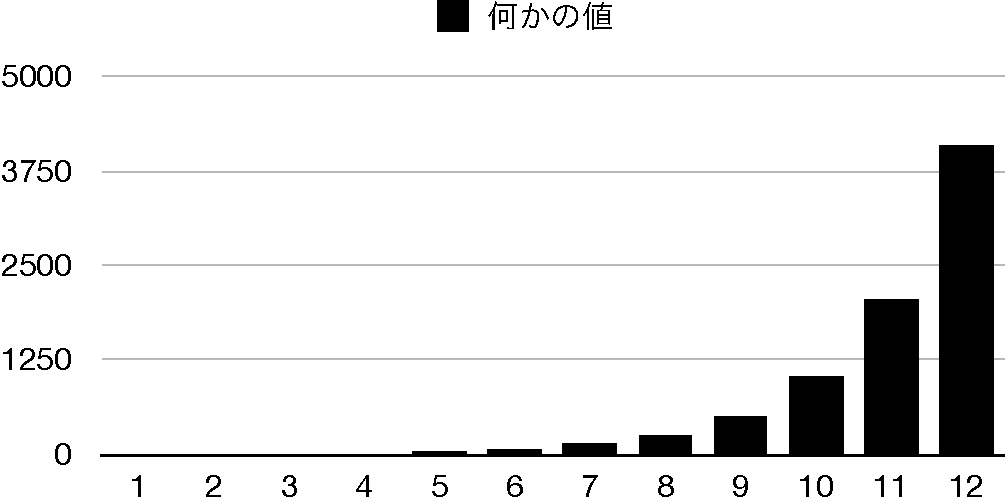
\includegraphics[width=0.9\textwidth]{examples/graphs/example}
  \caption{何かの値}\label{fig:example}
\end{figure}

\cref{fig:example}を見ると、何かの値が指数的に増加していることが分かる。
評価結果の詳細なデータを\cref{ch:appendix2}に示す。
      % サンプル
% \chapter{評価}\label{ch:evaluation}

\section{評価手法}\label{sec:methodology}

例えばここでは評価に用いたハードウェアやソフトウェアについて説明をする。
表を用いると効果的なことが多いので積極的に活用する。

\begin{table}[ht]
  \caption{数字が色々書いてある表}{
  \rowcolors{3}{gray90}{}
  \centering
  \resizebox{0.95\textwidth}{!}{
    {\renewcommand{\arraystretch}{1.3}
    \begin{tabular}{c>{\hspace{1pc}}c c c>{\hspace{1pc}}c c c} % https://tex.stackexchange.com/a/31704
      \toprule
      \multirow{2}{*}{比較対象} & \multicolumn{3}{c}{何かの結果} & \multicolumn{3}{c}{何かとの比較} \\
             & 面積($mm^2$) & 遅延($ns$) & 電力($m W$) & 面積(\%)  & 遅延(\%) & 電力(\%) \\
      \midrule
ベースライン &   347,329.19 &       1.62 &       15.84 &       --- &      --- &      --- \\
   提案手法1 &   412,263.87 &       1.65 &       16.17 &     18.69 &     1.85 &     2.12 \\
   提案手法2 &   370,972.35 &       2.42 &       17.95 &      6.80 &    49.38 &    11.00 \\
   提案手法3 &   356,694.82 &       1.98 &       16.00 &      2.69 &    22.22 &     1.06 \\
      \bottomrule
    \end{tabular}}\label{tab:example}
  }
}
\end{table}

\cref{tab:example}には色々な数字を示してある。
なお表には縦線を入れない方が見た目はすっきりしていて綺麗である(リンタの下記メッセージを見たことがある人もいるのではなかろうか:``Vertical rules in tables are ugly.'')。
また奇数列・偶数列の一方に網掛けを入れてある。
行数や列数が多い場合に視認性が高まるので適宜使うと良い。

\section{評価結果}\label{sec:results}

評価結果を定量的に示し、考察などを行なう。
グラフを用いること効果的なことが多いので積極的に活用する。

\begin{figure}[ht]
  \centering
  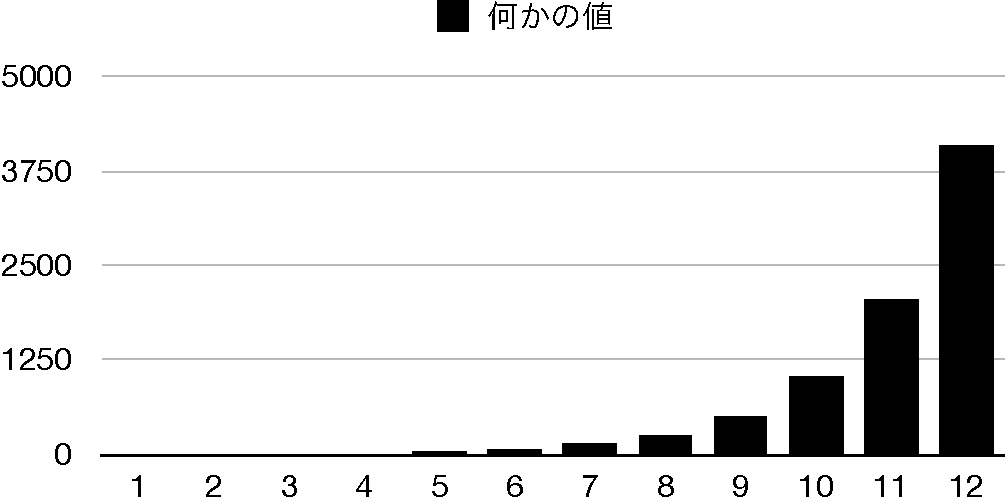
\includegraphics[width=0.9\textwidth]{examples/graphs/example}
  \caption{何かの値}\label{fig:example}
\end{figure}

\cref{fig:example}を見ると、何かの値が指数的に増加していることが分かる。
評価結果の詳細なデータを\cref{ch:appendix2}に示す。

\chapter{関連研究}\label{ch:relatedwork}

ここでは\cref{ch:background}に書くほど重要であったり密接に関係があるわけではないけれども、本研究を位置付ける(または俯瞰する)上で必要となる関連研究についてまとめる。
位置付けることが目的なので、本研究との差異がはっきりと分かるように関連研究の「関連した部分に関して」簡潔に記述する。     % サンプル
% \chapter{関連研究}\label{ch:relatedwork}

ここでは\cref{ch:background}に書くほど重要であったり密接に関係があるわけではないけれども、本研究を位置付ける(または俯瞰する)上で必要となる関連研究についてまとめる。
位置付けることが目的なので、本研究との差異がはっきりと分かるように関連研究の「関連した部分に関して」簡潔に記述する。
\chapter{結論}\label{ch:conclusion}

本研究で何をなぜやったのか、その結果何が分かったのかを記述する。
将来的にどのように本研究を発展させられるか、なども書いて良いかもしれない。      % サンプル
% \chapter{結論}\label{ch:conclusion}

本研究で何をなぜやったのか、その結果何が分かったのかを記述する。
将来的にどのように本研究を発展させられるか、なども書いて良いかもしれない。
\chapter*{謝辞}
\addchapter{謝辞}

肩肘はらずに普通に感謝の言葉を述べるくらいで良いと思われる。  % サンプル
% \chapter*{謝辞}
\addchapter{謝辞}

肩肘はらずに普通に感謝の言葉を述べるくらいで良いと思われる。
\bibliographystyle{junsrt}
\bibliography{examples/main}       % サンプル
% \bibliography{main}
\appendix

\chapter{定理1の証明}\label{ch:appendix1}

\chapter{\cref{sec:results}の詳細なデータ}\label{ch:appendix2}          % サンプル
% \appendix

\chapter{定理1の証明}\label{ch:appendix1}

\chapter{\cref{sec:results}の詳細なデータ}\label{ch:appendix2}

\end{document}